\documentclass[border=3pt]{standalone}
% Shared preamble for standalone TikZ figures (colors match the slide theme).
\usepackage[T1]{fontenc}
\IfFileExists{sourcesanspro.sty}{\usepackage[default]{sourcesanspro}}{\usepackage[scaled=0.92]{helvet}\renewcommand{\familydefault}{\sfdefault}}
\usepackage{xcolor,tikz}
\usetikzlibrary{arrows.meta,positioning,calc,shapes.geometric,decorations.pathmorphing,decorations.pathreplacing,backgrounds,fit}
\definecolor{fsNavy}{HTML}{1B365D}
\definecolor{fsAccent}{HTML}{C8102E}
\definecolor{fsGold}{HTML}{D39B1E}
\definecolor{fsTeal}{HTML}{1F7A8C}
\definecolor{fsGreen}{HTML}{3A7D44}
\definecolor{fsGray}{HTML}{5B6770}
\definecolor{fsLight}{HTML}{EEF2F6}
\tikzset{
  molbox/.style={draw=black!55,rounded corners=3pt,line width=0.6pt,
                 minimum height=7mm,font=\small\bfseries,inner xsep=3mm},
  site/.style={circle,draw=black!55,fill=white,inner sep=0pt,minimum size=4mm,
               font=\tiny\bfseries,line width=0.5pt},
  psite/.style={site,fill=fsAccent,text=white},
  bond/.style={line width=1.3pt,black!70},
  callout/.style={font=\scriptsize,text=fsGray,align=left},
  pointer/.style={-{Stealth[length=1.6mm]},fsGray,line width=0.5pt},
}
\newcommand{\code}[1]{{\ttfamily #1}}

\begin{document}
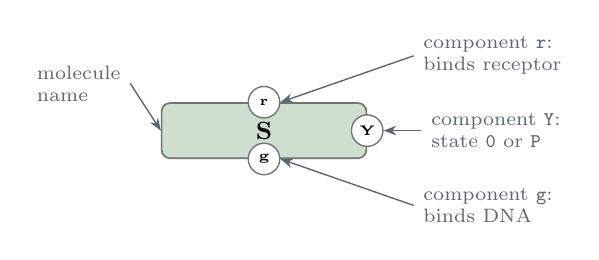
\begin{tikzpicture}[x=1cm,y=1cm]
  \node[molbox,fill=fsGreen!25,minimum width=2.6cm] (S) at (0,0) {S};
  \node[site] (r) at ($(S.north)$) {r};
  \node[site] (Y) at ($(S.east)$) {Y};
  \node[site] (g) at ($(S.south)$) {g};
  \node[callout,anchor=west] (cr) at (1.9,0.95) {component \code{r}:\\binds receptor};
  \draw[pointer] (cr.west) -- (r.east);
  \node[callout,anchor=west] (cY) at (2.0,0) {component \code{Y}:\\state \code{0} or \code{P}};
  \draw[pointer] (cY.west) -- (Y.east);
  \node[callout,anchor=west] (cg) at (1.9,-0.95) {component \code{g}:\\binds DNA};
  \draw[pointer] (cg.west) -- (g.east);
  \node[callout,anchor=east] (cm) at (-1.7,0.6) {molecule\\name};
  \draw[pointer] (cm.east) -- (S.west);
\end{tikzpicture}
\end{document}
